\documentclass{article}

\usepackage{Sweave}
\begin{document}
\Sconcordance{concordance:aula03a.tex:aula03a.Rnw:%
1 2 1 1 0 4 1 1 3 1 0 6 1 1 3 2 1 1 2 3 1 1 2 1 1 2 2 1 1 1 9 7 0 1 2 4 %
0 1 2 1 1}


\section{Aula 4 - 23/03/2018}

\begin{Schunk}
\begin{Sinput}
>   library('plot3D')
>   rm(list = ls())
>   xc1<-matrix(rnorm(100,sd=0.4),ncol=2)+2
>   xc2<-matrix(rnorm(100,sd=0.4),ncol=2)+4
>   plot(xc1[,1],xc1[,2],col='red',xlim=c(0,6),ylim=c(0,6),xlab='',ylab='')
>   par(new=T)
>   plot(xc2[,1],xc2[,2],col='blue',xlim=c(0,6),ylim=c(0,6),xlab='',ylab='')
>   w1<-1
>   w2<-1
>   theta<-6
>   fx1<-seq(0,6,0.1);
>   fx2<--w1/w2*fx1+theta/w2
>   par(new=T)
>   plot(fx1,fx2,col='black',type='l')
>   seqi<-seq(0,6,0.1)
>   seqj<-seq(0,6,0.1)
>   M<-matrix(1,nrow=length(seqi),ncol=length(seqj))
>   ci<-0
>   cj<-0
>   for(i in seqi) {
+     ci<-ci+1
+     cj<-0
+     for(j in seqj) {
+       cj<-cj+1
+       M[ci,cj]<-1*(i*w1+j*w2>=theta)
+     }
+   }
>   persp3D(seqi,seqj,M)
\end{Sinput}
\end{Schunk}
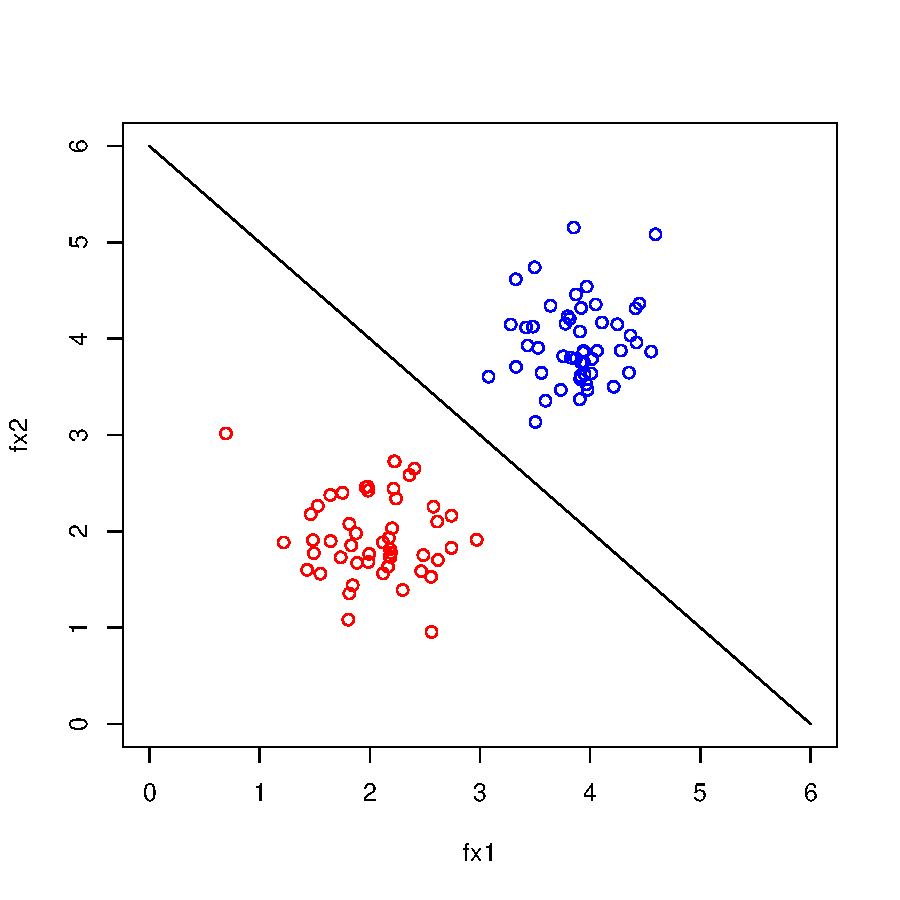
\includegraphics{aula03a-001}

\end{document}
